\section{Class\-One Class Reference}
\label{classClassOne}\index{ClassOne@{ClassOne}}
Inheritance diagram for Class\-One::\begin{figure}[H]
\begin{center}
\leavevmode
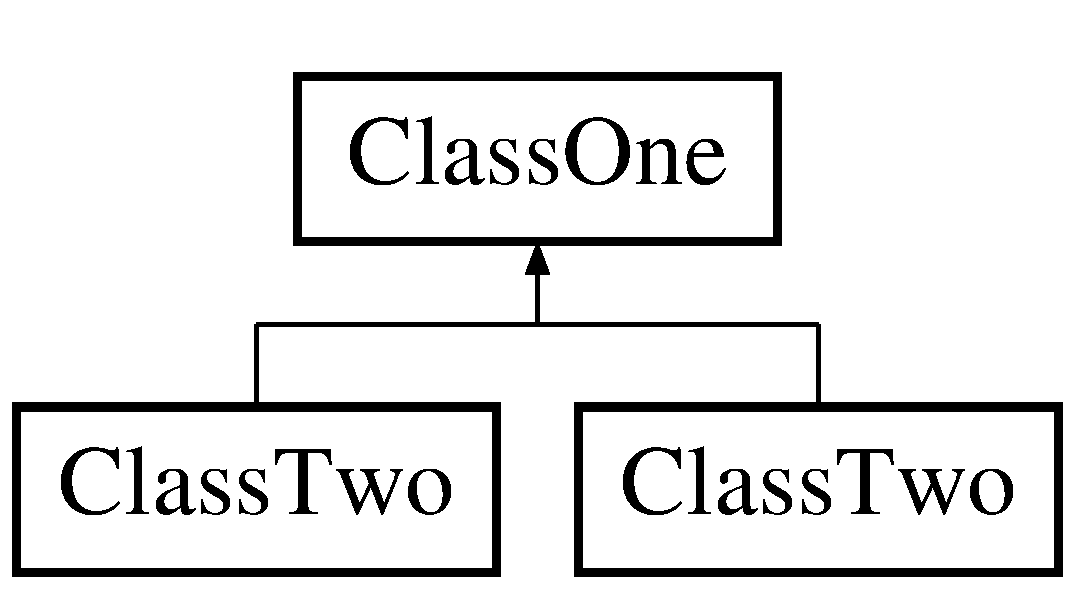
\includegraphics[height=2cm]{classClassOne}
\end{center}
\end{figure}
\subsection*{Public Member Functions}
\begin{CompactItemize}
\item 
int {\bf member\-Static} ()\label{classClassOne_82562b89ee05aaaea678c8d03195c4fa}

\item 
int {\bf member} ()\label{classClassOne_2891d675a1a24cbefb4d137c7a6c5246}

\item 
abstract int {\bf abstract\-Member} ()\label{classClassOne_d4d6e41c525f13b52ac972e78617670f}

\item 
{\bf Class\-One} ()\label{classClassOne_a3e3a578984311bf8d06c453be8e4bf7}

\end{CompactItemize}
\subsection*{Static Public Member Functions}
\begin{CompactItemize}
\item 
static int {\bf static\-Member} ()\label{classClassOne_3dcd89d59ceccfeb86b8d59cb50cac28}

\item 
static void {\bf initialize} ({\bf Class\-One} one, String field\-Name)\label{classClassOne_72359492bd342810d4036c367c6b3c9d}

\end{CompactItemize}
\subsection*{Static Public Attributes}
\begin{CompactItemize}
\item 
static String {\bf one\-Data}\label{classClassOne_b5c7fc191be97409dd14e61c55d30c44}

\item 
static boolean {\bf initialized} = false\label{classClassOne_c0cbceb167235a8176162c91b1799f59}

\end{CompactItemize}
\subsection*{Package Attributes}
\begin{CompactItemize}
\item 
int {\bf number} = {\bf NUMBER}\label{classClassOne_20ec65c5bc52a2f84ee38f70816ec999}

\item 
int {\bf member\-Number} = 1\label{classClassOne_f694a5edfcf9acd7b65a6befb38a5815}

\end{CompactItemize}
\subsection*{Static Package Attributes}
\begin{CompactItemize}
\item 
static int {\bf NUMBER} = 1\label{classClassOne_2ea5ab820741736b25aac6903be8464c}

\end{CompactItemize}


\subsection{Detailed Description}




Definition at line 50 of file Test\-Static\-Inheritance.java.

The documentation for this class was generated from the following files:\begin{CompactItemize}
\item 
Test\-Static\-Inheritance.java\item 
Test\-Static\-Initializer.java\end{CompactItemize}
